\documentclass[dvipsnames]{beamer}
\usepackage{lmodern}
\usepackage{appendixnumberbeamer}
\renewcommand{\sfdefault}{lmss}
\renewcommand{\ttdefault}{lmtt}
\usepackage[T1]{fontenc}
% \usepackage[utf8]{inputenc}
\setcounter{secnumdepth}{3}
\setcounter{tocdepth}{3}
\usepackage{amsmath}
\usepackage{amsthm}
\usepackage{amssymb}
\theoremstyle{definition}
\newtheorem*{defn*}{\protect\definitionname}
\providecommand{\definitionname}{Definition}
\usepackage{graphicx}
\usepackage{hyperref}
\usepackage{ulem}
\PassOptionsToPackage{normalem}{ulem}
\usepackage{caption}
\usepackage{subcaption}
\usepackage{verbatim}
\usepackage[english]{babel}
\usepackage[autostyle]{csquotes}
\usepackage{tikz}
\usetikzlibrary{arrows,intersections}
\usepackage{pgfplots}
\pgfplotsset{compat = 1.15}
\usepgfplotslibrary{fillbetween}
\usepackage{verbatim}
\usepackage{booktabs}
\usepackage{multirow}
\usepackage{array}
\usepackage{nccmath}
% \usepackage{listings}
\usepackage{mathtools}

%Bibliography style, etc.
\usepackage[citestyle=authoryear-comp,natbib, uniquename = false, url = false, doi = false, uniquelist=false]{biblatex}
\renewbibmacro{in:}{}
\AtEveryBibitem{%
  \clearfield{volume}%
  \clearfield{number}
  \clearfield{month}
  \clearfield{issn}
  \clearfield{isbn}
  \clearfield{pages}
}

%\usepackage{cleveref}
\usepackage{setspace}
\makeatletter

% Macros
\providecommand{\tabularnewline}{\\}
\newcommand{\gr}{\textcolor{ForestGreen}} 
\newcommand{\rd}{\textcolor{red}}
\newcommand{\cb}{\textcolor{CornflowerBlue}} %this is the blue color you like; simply type \cb{X} where "X" is the color you want in blue
\newcommand{\vitem}{\vfill \item} %auto-centers items in lists
\newcommand{\fall}{\ \forall} %redefines "forall" (I don't like the default spacing)
\newcommand{\frall}{\quad \forall} %a \forall separated from the main math; this is the way it usually shows up in equations
\newcommand{\exist}{\ \exists} %same as \fall, but for \exists; they have the same ugly spacing
\newcommand{\R}{\mathbb{R}} %set of real numbers
\newcommand*\bigcdot{\mathpalette\bigcdot@{.5}} %different size for cdots
% \newcommand{\argmax}{\text{arg}\max}
\newenvironment{itemframe}
    {\frame{}\itemize}
    {\itemize\frame}
\newcommand\makebeamertitle{\frame{\maketitle}}%
\newtheoremstyle{named}{}{}{\itshape}{}{\bfseries}{.}{.5em}{\thmnote{#3's }#1}
\theoremstyle{named}
\newtheorem*{prop*}{Proposition}
% \newtheorem*{corollary}{Corollary}
\newtheorem*{namedtheorem}{Theorem} %allows named theorems
\newtheorem*{nameddef}{Definition}
\newtheorem{proposition}{Proposition}
\newtheorem*{assumption}{Assumption}
\newtheorem*{namedcorollary}{Corollary}
\newtheorem*{namedlemma}{Lemma}
\newtheorem*{axiom}{Axiom}
\newtheorem*{theorem*}{Theorem}
\newtheorem*{lemma*}{Lemma}
\DeclareMathOperator*{\argmin}{argmin}
\DeclareMathOperator{\argmax}{argmax}
\DeclareMathOperator{\supp}{supp}
\DeclareMathOperator{\interior}{int}
\DeclareMathOperator{\rank}{rank}
\newcolumntype{C}[1]{>{\centering\let\newline\\\arraybackslash\hspace{0pt}}m{#1}}
\newcommand{\sbt}{\,\begin{picture}(-1,1)(-1,-3)\circle*{2}\end{picture}\ }



%formatting
\usetheme{Ilmenau}
\definecolor{MIT}{rgb}{.639,.122,.204}
\definecolor{UCLA}{rgb}{0.15294117647058825, 0.4549019607843137, 0.6823529411764706}
\definecolor{UCLA_gold}{rgb}{1, 0.8196078431372549, 0}
\usecolortheme[named=UCLA]{structure}
\setbeamercolor*{palette secondary}{fg=UCLA_gold,bg=gray!15!white}
\usecolortheme{dolphin}
\setbeamertemplate{navigation symbols}{} 
\setbeamertemplate{footline}{}{}
\setbeamertemplate{headline}{}
\setbeamertemplate{navigation symbols}{}
\mode<presentation> {}
\setbeamercolor{block title}{use=structure,fg=white,bg=RoyalBlue} %blocks (theorems, etc.)in blue
\setbeamercolor{block title alerted}{use=structure,fg=white,bg=ForestGreen} %blocks (theorems, etc.)in blue

\renewcommand\qedsymbol{$\blacksquare$} %set QED symbol as black square
\renewcommand{\emph}{\textit} %set emphasized text style; this is italics
\setbeamertemplate{footline}[frame number] %slide numbers
\setbeamertemplate{itemize item}[circle] %bullet style
\setbeamertemplate{itemize subitem}{--}
\setbeamertemplate{enumerate item}[default]
\newrobustcmd*{\parentexttrack}[1]{%
  \begingroup
  \blx@blxinit
  \blx@setsfcodes
  \blx@bibopenparen#1\blx@bibcloseparen
  \endgroup}

\AtEveryCite{%
  \let\parentext=\parentexttrack%
  \let\bibopenparen=\bibopenbracket%
  \let\bibcloseparen=\bibclosebracket}

 \AtBeginDocument{%
   \let\origtableofcontents=\tableofcontents
   \def\tableofcontents{\@ifnextchar[{\origtableofcontents}{\gobbletableofcontents}}
   \def\gobbletableofcontents#1{\origtableofcontents}
 }
\newcommand{\backupbegin}{
   \newcounter{framenumberappendix}
   \setcounter{framenumberappendix}{\value{framenumber}}
}
\newcommand{\backupend}{
   \addtocounter{framenumberappendix}{-\value{framenumber}}
   \addtocounter{framenumber}{\value{framenumberappendix}} 
} 

\renewcommand{\maketitle}{
\setbeamertemplate{footline}{} 
\begin{frame}[noframenumbering]
\titlepage
\end{frame}
\setbeamertemplate{footline}[frame number]
}

\usefonttheme[onlymath]{serif}

% \usetheme{CambridgeUS}

% \newtheorem{theorem}{Theorem}
% \theoremstyle{claim}
\newtheorem{claim}{Claim}
% \newtheorem{corollary}{Corollary}


\makeatother


%\author{Drew Fudenberg}

\institute[]{}
\title{Understanding the Price Effects of the MillerCoors Joint Venture}
\author{Miller, Weinberg (2017)}
\begin{document}
\maketitle
%
\begin{frame}{Overview}
  \begin{itemize}
  \item Miller and Coors merged; why did the FTC let them?
    \vitem What does economic theory say about how Miller and Coors will behave post-merger?
    \vitem What does economic theory say about how \emph{other} firms will behave post-merger?
    \vitem Authors have very detailed sales data.
    \vitem \textbf{Research Question:} Are the firms competing \`a la Nash-Bertrand post-merger?
    \begin{itemize}
    \item Spoiler: No.
    \item Harder question: \emph{How} are firms colluding, and which firms?
        \item More interesting question: Why did the FTC approve this merger?
    \end{itemize}
  \end{itemize}
\end{frame}
%
\begin{frame}{Market Overview}
  \begin{center}
   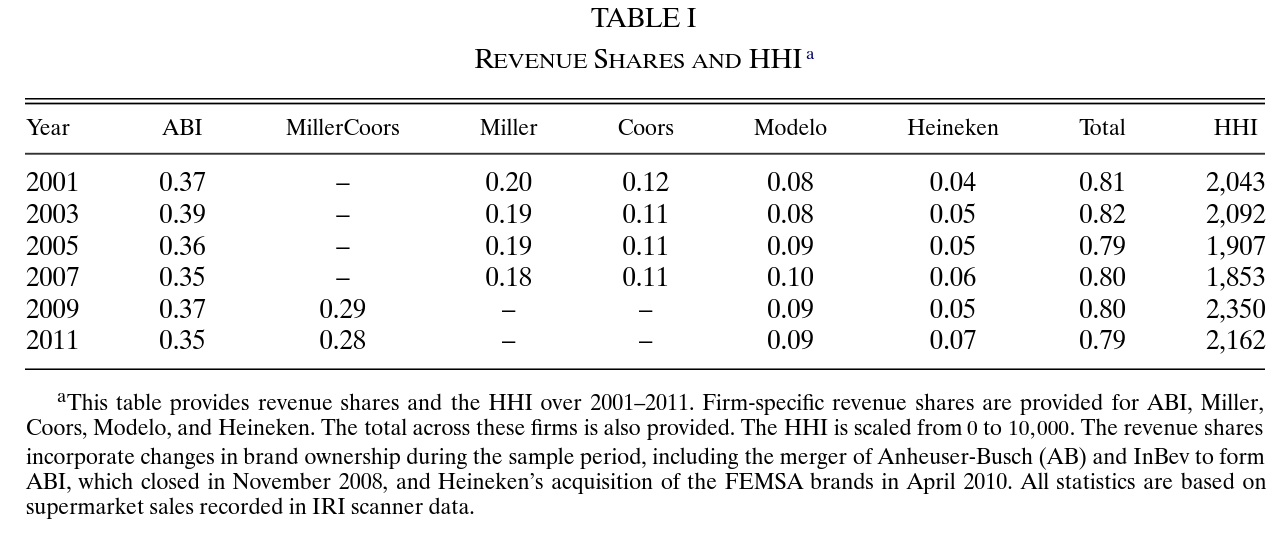
\includegraphics[width=\textwidth, keepaspectratio=true]{tab1.png} 
  \end{center}
  \begin{itemize}
  \item Recall that merger guidelines say that HHI $\in$ (1500, 2500) is a gray area; needs further consideration
  \end{itemize}
\end{frame}
%
\begin{frame}{Descriptive Smoking Gun}
  \begin{center}
    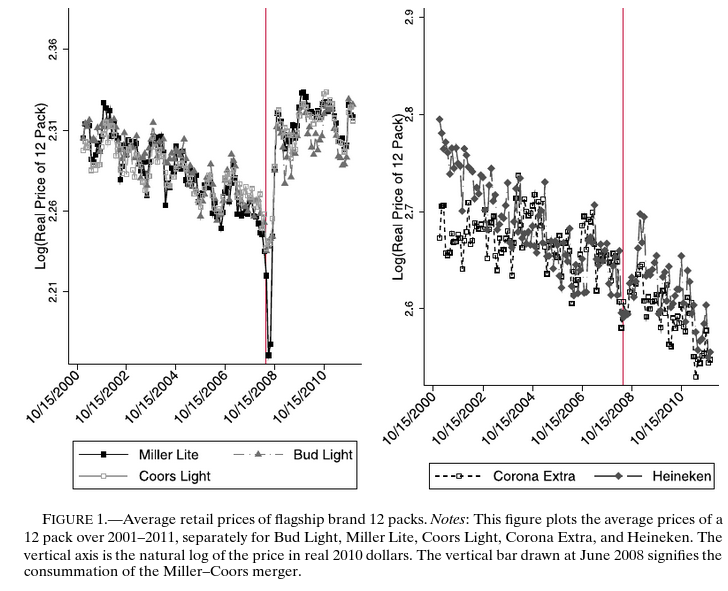
\includegraphics[width=0.9\textwidth, keepaspectratio=true]{fig1.png}
  \end{center}
\end{frame}
%
\begin{frame}{Demand}
  \begin{itemize}
  \item Model consumer demand using Random Coefficient Nested Logit (RCNL)
  \[
s_{jrt} = \frac{1}{N_{rt}}\sum^{N_{rt}}_{i = 1} \frac{\exp\left((\delta_{jrt} + \mu_{ijrt})/(1 - \rho)\right)}{\exp\left(I_{igrt}/(1 - \rho)\right)} \frac{\exp I_{igrt}}{\exp I_{irt}}
  \]
  \[
  \begin{array}[l]{lcl}
    \rho &\equiv & \text{ nesting parameter} \\
    \delta & \equiv & \text{ mean utility}\\
    \mu & \equiv & \text{ consumer-specific deviations}
  \end{array}
  \]
    \vitem This relaxes some restrictions on substitution patterns and allows for ``natural'' economic impacts, e.g. from the recession
\vitem This approach is pretty common in empirical IO (Asker 2016)
  \end{itemize}
\end{frame}
%
\begin{frame}{Estimation and Instruments}
  \begin{itemize}
  \item Estimation via GMM
    \[
\hat{\theta}^D = \arg \min_\theta \omega(\theta)^\prime Z A^{-1}Z^\prime \omega (\theta)
    \]
    \item Identification requires one instrument for price, and an instrument for each non-linear parameter
    \vitem \textbf{Price Instruments (supply side)}
    \begin{enumerate}
    \item Distance between the brewery and region
      \item Indicator for ABI and MillerCoors products post-merger
    \end{enumerate}
    \vitem \textbf{Instruments for the nesting parameter}
    \begin{enumerate}
      \item[---] Need exogenous variation in the conditional shares of the inside goods
    \item Number of products in the market
      \item Distance summed across products in the marke
    \end{enumerate}
  \end{itemize}
\end{frame}
%
\begin{frame}{}
  \begin{center}
    \vspace{-1em}
    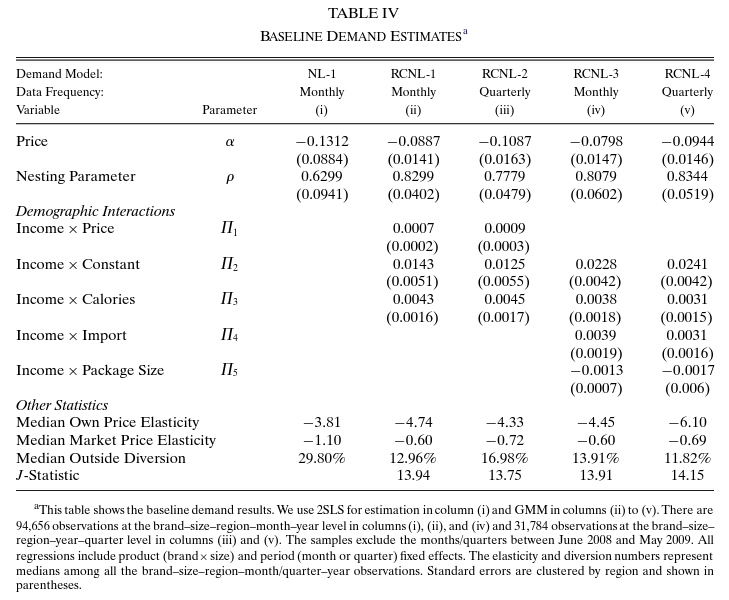
\includegraphics[height=\textheight, keepaspectratio=true]{tab4.png}
  \end{center}
\end{frame}
%
\begin{frame}{Supply Model}
  \begin{itemize}
  \item Differentiated-products price competition
    \vitem Post-merger, ABI and/or MillerCoors partially internalize their pricing externalities
    \[
      \Omega_{t^\ast_1} = \underbrace{\begin{bmatrix}
        1 & 0 & 0 & 0\\
        0 & 1 & 0 & 0\\
        0 & 0 & 1 & 0\\
        0 & 0 & 0 & 1
      \end{bmatrix}}_{\text{Nash-Bertrand}} \qquad \Omega_{t^\ast_2} =
    \underbrace{\begin{bmatrix}
      1 & \rd{\kappa} & \rd{\kappa} & 0\\
      \rd{\kappa} & 1 & \gr{1} & 0\\
      \rd{\kappa} & \gr{1} & 1 & 0\\
      0 & 0 & 0 & 1
    \end{bmatrix}}_{\text{post-merger}}
    \]
    \vitem \gr{Green} terms capture full internalization by MillerCoors
    \vitem $\rd{\kappa}$ captures partial internalization due to collusion between ABI and MillerCoors
    \vitem We still have 0's in some places because Modelo doesn't get to collude
  \end{itemize}
\end{frame}
%
\begin{frame}{Supply Estimates}
  \begin{center}
    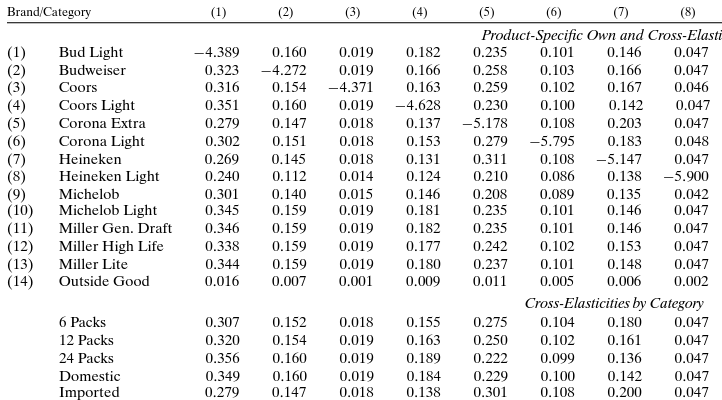
\includegraphics[height=0.7\textheight, keepaspectratio=true]{elasticities.png}
  \end{center}
\end{frame}
%
\begin{frame}{ABI/MillerCoors $\ne$ Modelo}
  \begin{center}
   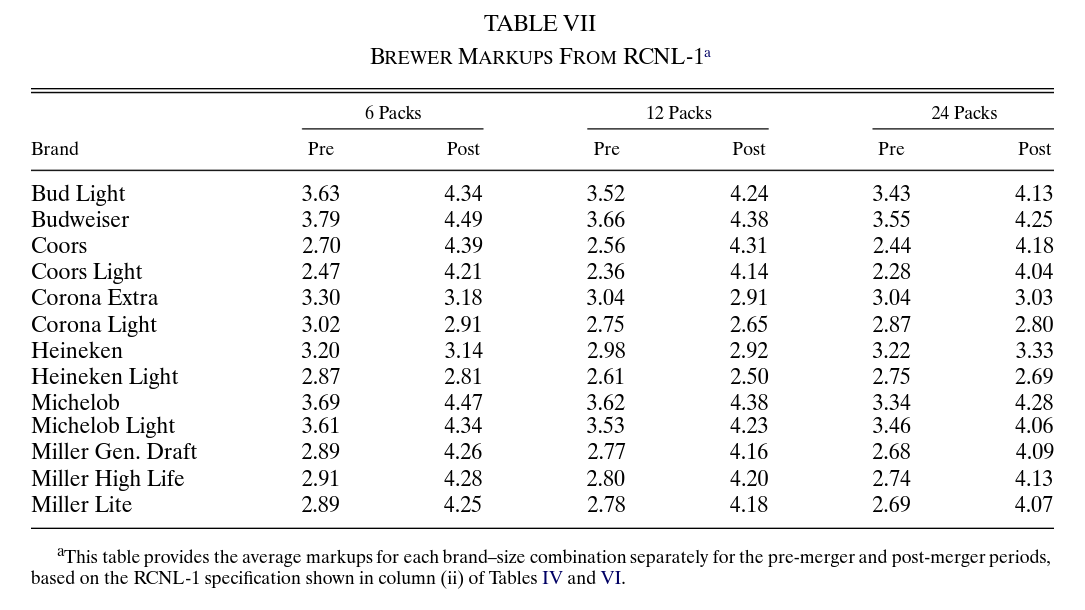
\includegraphics[width=\textwidth, keepaspectratio=true]{tab7.png} 
  \end{center}
\end{frame}
%
\begin{frame}{But\ldots what if they weren't colluding?}
  \begin{center}
    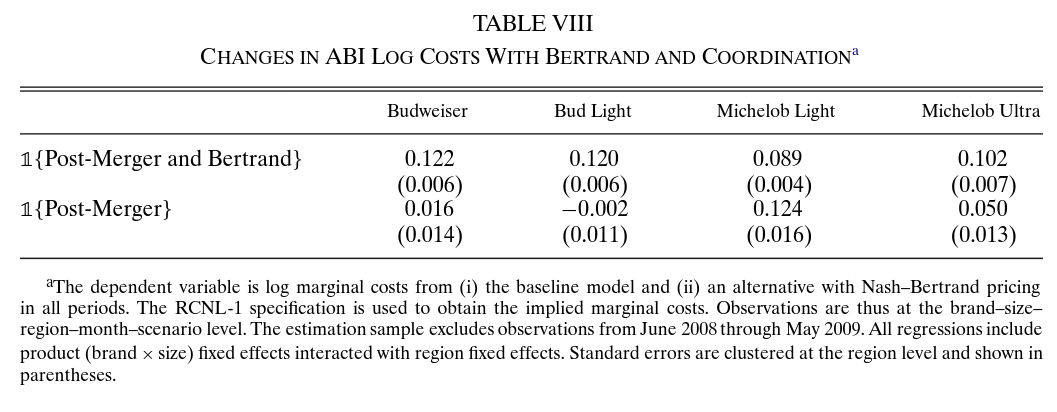
\includegraphics[width=\textwidth, keepaspectratio=true]{tab8.png}
  \end{center}
  \begin{itemize}
  \item Seems unlikely that ABI had costs skyrocket for no apparent reason
    \vitem However, much harder to say that the merger between Miller and Coors \emph{caused} the switch in competition/firm conduct
  \end{itemize}
\end{frame}
%
\begin{frame}{So, why did the FTC approve the merger?}
  \begin{center}
    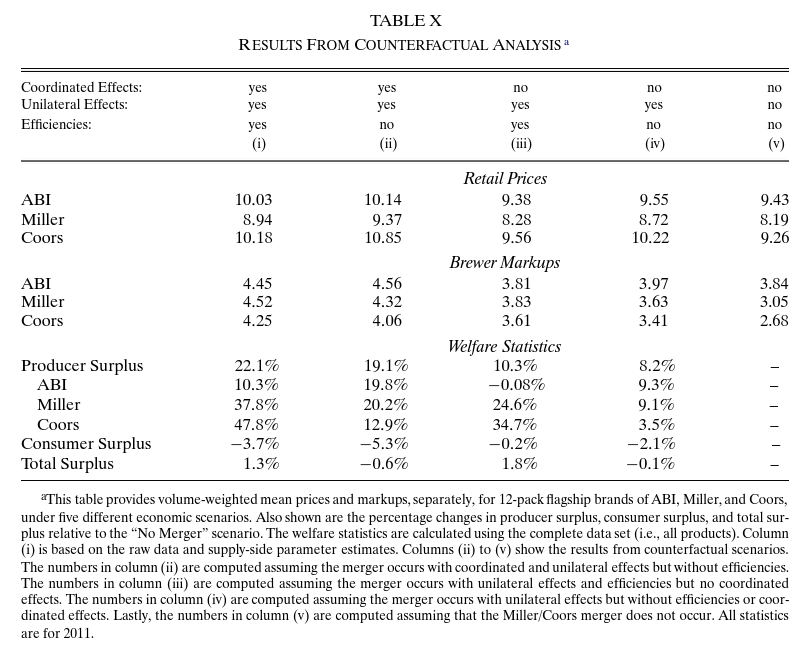
\includegraphics[width=0.9\textwidth, keepaspectratio=true]{tab10.png}
  \end{center}
\end{frame}
\end{document}
%%% Local Variables:
%%% mode: latex
%%% TeX-master: t
%%% End:
